\chapter{Evaluation \& Testing}\label{ch:Evaluation}

This chapter presents the experimental results, provides a comparative analysis of all forecasting models, examines feature importance, and dThe evaluation demonstrates that the CatBoost-PPSO model achieves the best predictive performance among all tested model configurations, with an $R^2$ of 0.914, MAE of 1{,}496.2 MWh, and MAPE of 0.89\%. PPSO optimisation provides a consistent $\sim$10\% improvement over default CatBoost across all error metrics, a smaller gain for XGBoost, and no gain for Random Forest---evidence that the fair, uniform tuning protocol correctly isolates algorithmic merit. Feature importance analysis confirms that autoregressive demand features are the strongest predictors, with temperature and temporal calendar features providing important supplementary signal. These results validate the applicability of the hybrid CatBoost-PPSO methodology to daily national-level demand forecasting in a tropical climate.scusses the findings in the context of the research objectives.


\section{Experimental Setup}

All models were trained on the same 852-sample training set and evaluated on the 213-sample held-out test set using the six metrics defined in Section~\ref{sec:eval_metrics}. To ensure a fair comparison, PPSO optimisation was applied to \emph{every} tree-based model (Random Forest, XGBoost, and CatBoost) under an identical budget: 15 particles over 20 iterations, with 3-fold \texttt{TimeSeriesSplit} cross-validation as the fitness function. All random seeds were fixed to 42 for reproducibility.


\section{Model Comparison Results}

Table~\ref{tab:model_comparison} presents the performance of all models on the test set, sorted by RMSE (ascending).

\begin{table}[H]
\centering
\caption{Model comparison on the test set (213 samples). Models are sorted by RMSE. Best values in each column are shown in \textbf{bold}.}
\label{tab:model_comparison}
\begin{tabular}{@{}lrrrrrr@{}}
\toprule
\textbf{Model} & \textbf{MAE} & \textbf{RMSE} & \textbf{$R^2$} & \textbf{MAPE (\%)} & \textbf{RAE} & \textbf{WI} \\
\midrule
CatBoost-PPSO & \textbf{1{,}496.2} & \textbf{1{,}895.5} & \textbf{0.9135} & \textbf{0.89} & \textbf{0.280} & \textbf{0.9774} \\
CatBoost & 1{,}679.4 & 2{,}118.8 & 0.8919 & 0.99 & 0.314 & 0.9709 \\
Linear Reg. & 1{,}693.4 & 2{,}119.2 & 0.8919 & 1.01 & 0.317 & 0.9731 \\
XGB-PPSO & 1{,}687.8 & 2{,}165.6 & 0.8871 & 1.00 & 0.315 & 0.9697 \\
Random Forest & 1{,}774.0 & 2{,}237.6 & 0.8795 & 1.05 & 0.332 & 0.9653 \\
RF-PPSO & 1{,}794.1 & 2{,}283.9 & 0.8744 & 1.06 & 0.335 & 0.9634 \\
XGBoost & 1{,}833.4 & 2{,}313.4 & 0.8712 & 1.08 & 0.343 & 0.9652 \\
\bottomrule
\end{tabular}
\end{table}

\subsection{Key Observations}

\begin{enumerate}
    \item \textbf{CatBoost-PPSO achieves the best performance across all six metrics.} Its $R^2$ of 0.914 indicates that the model explains over 91\% of the variance in daily electricity demand. The RMSE of 1{,}895.5 MWh represents approximately 1.1\% of the mean daily demand, and the MAPE of 0.89\% confirms excellent relative accuracy.
    
    \item \textbf{PPSO benefits are model-dependent.} For CatBoost, PPSO tuning improves MAE by 10.9\% (1{,}679 $\to$ 1{,}496) and RMSE by 10.5\% (2{,}119 $\to$ 1{,}896). For XGBoost, PPSO also helps substantially (RMSE 2{,}313 $\to$ 2{,}166, $-$6.4\%). For Random Forest, however, PPSO tuning slightly degrades test performance (RMSE 2{,}238 $\to$ 2{,}284), indicating mild overfitting of the cross-validated fitness to the training period. Applying PPSO to all tree models under the same budget makes these differences visible and confirms that CatBoost-PPSO's lead is not merely an artefact of preferential tuning.
    
    \item \textbf{Linear Regression performs surprisingly well}, essentially tied with default CatBoost on RMSE and $R^2$. This suggests that the relationship between the engineered features and demand is substantially linear, likely driven by the strong autoregressive features (lag-1 and rolling means). However, Linear Regression cannot capture interaction effects between weather and temporal variables.
    
    \item \textbf{Random Forest and XGBoost occupy the lower ranks} in their default configurations, and both are clearly outperformed by CatBoost-PPSO, suggesting that native categorical handling combined with PPSO-tuned hyperparameters provides genuine advantages.
    
    \item \textbf{All models achieve $R^2 > 0.87$ and WI $> 0.96$}, indicating that the 16-feature set captures the dominant drivers of electricity demand effectively.
\end{enumerate}

\begin{figure}[H]
    \centering
    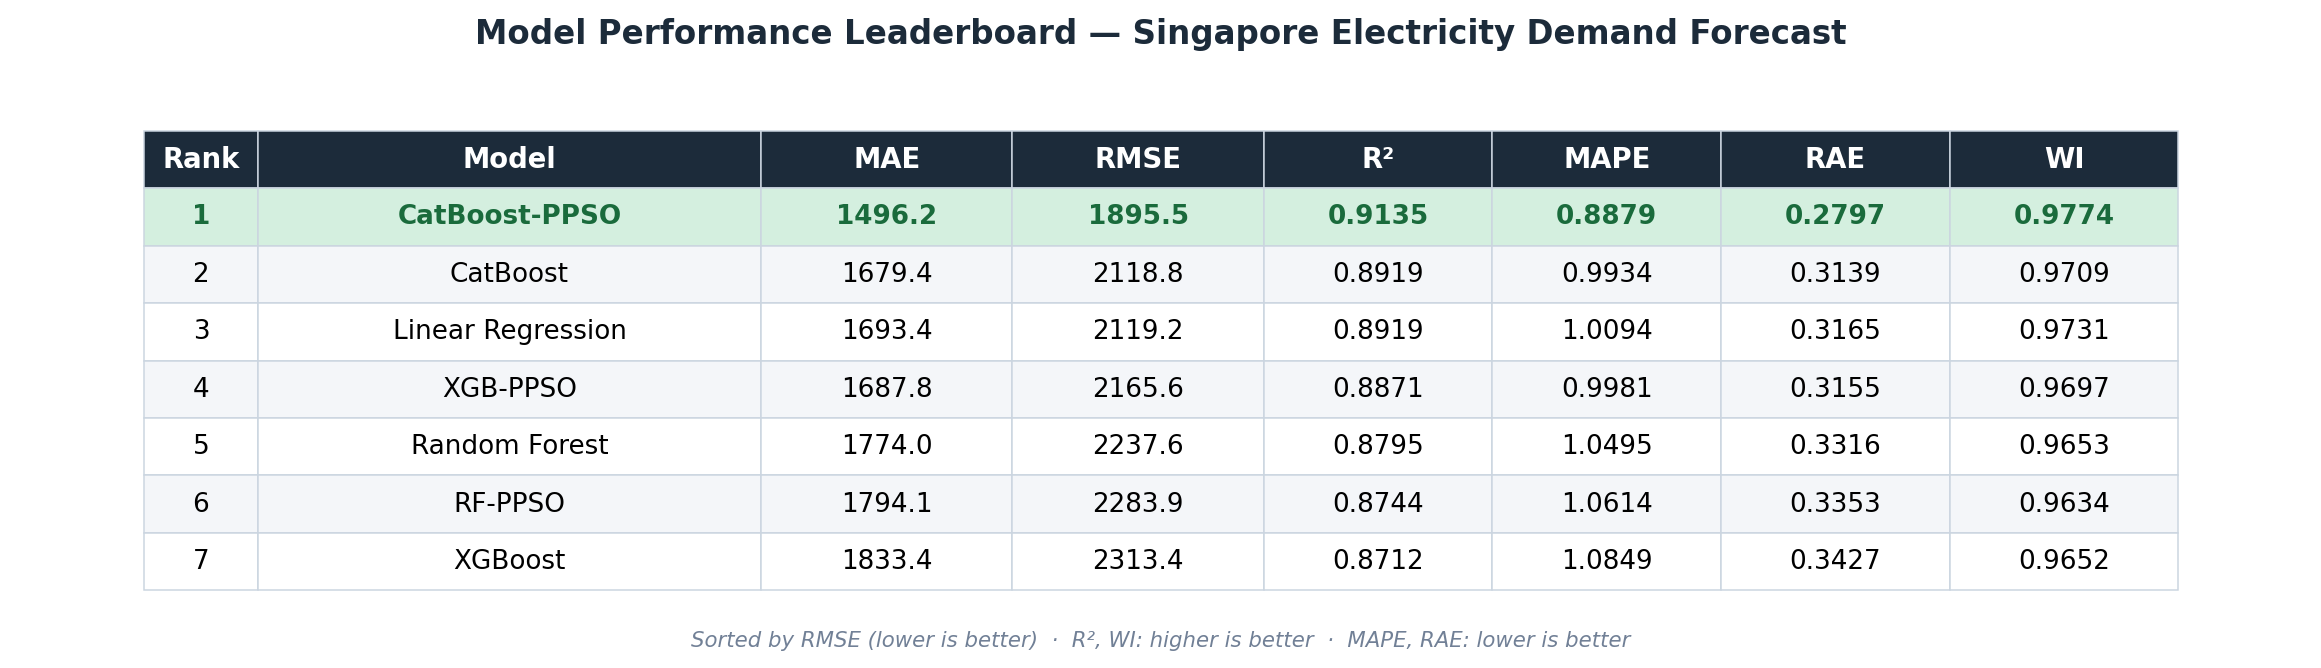
\includegraphics[width=0.90\textwidth]{eval/images/model_comparison_table.png}
    \caption{Visual comparison of model performance metrics. CatBoost-PPSO (top row) achieves the best scores across all metrics.}
    \label{fig:model_comparison_visual}
\end{figure}


\section{Prediction Analysis}

Figure~\ref{fig:predictions} shows the actual versus predicted daily electricity demand for the CatBoost-PPSO model on the test set.

\begin{figure}[H]
    \centering
    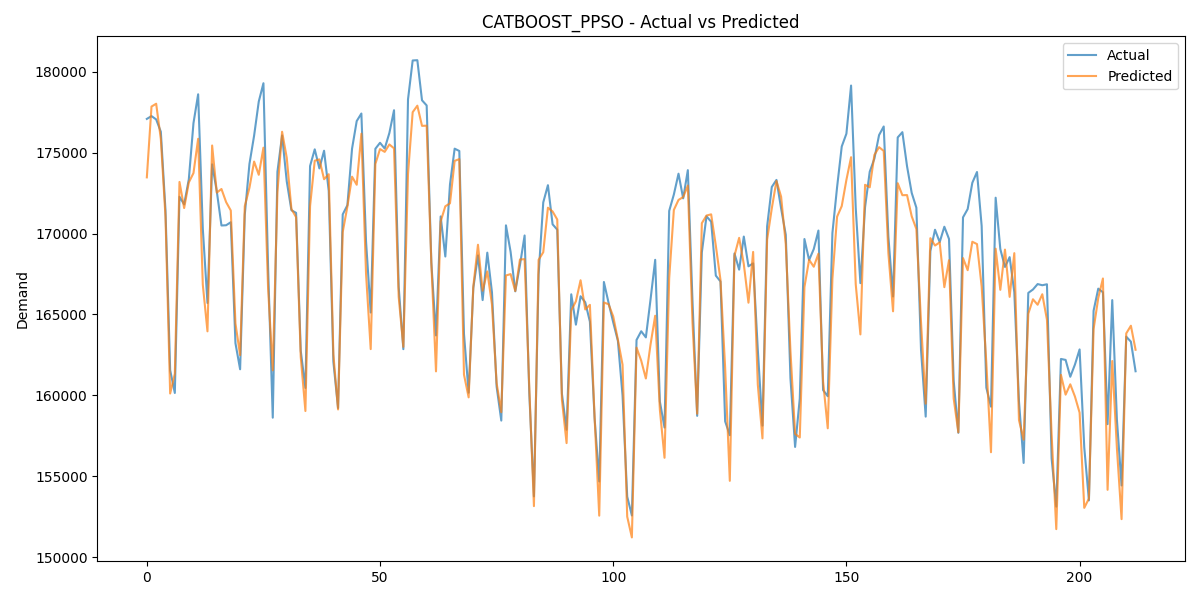
\includegraphics[width=0.95\textwidth]{eval/images/predictions_catboost_ppso.png}
    \caption{Actual vs.\ predicted daily electricity demand (MWh) for the CatBoost-PPSO model on the test set (213 days). The model closely tracks both the overall demand trend and short-term fluctuations.}
    \label{fig:predictions}
\end{figure}

The prediction plot reveals that CatBoost-PPSO captures:
\begin{itemize}
    \item \textbf{Weekly cyclicity}: The regular dips on weekends are accurately reproduced.
    \item \textbf{Demand level shifts}: Transitions between higher and lower demand periods are tracked.
    \item \textbf{Occasional outliers}: Some extreme demand drops (likely associated with public holidays) show slightly larger prediction errors, but the overall tracking is tight.
\end{itemize}


\section{Feature Importance Analysis}

Feature importance was extracted from the CatBoost-PPSO model's underlying CatBoost estimator using built-in feature importance scores.

\begin{figure}[H]
    \centering
    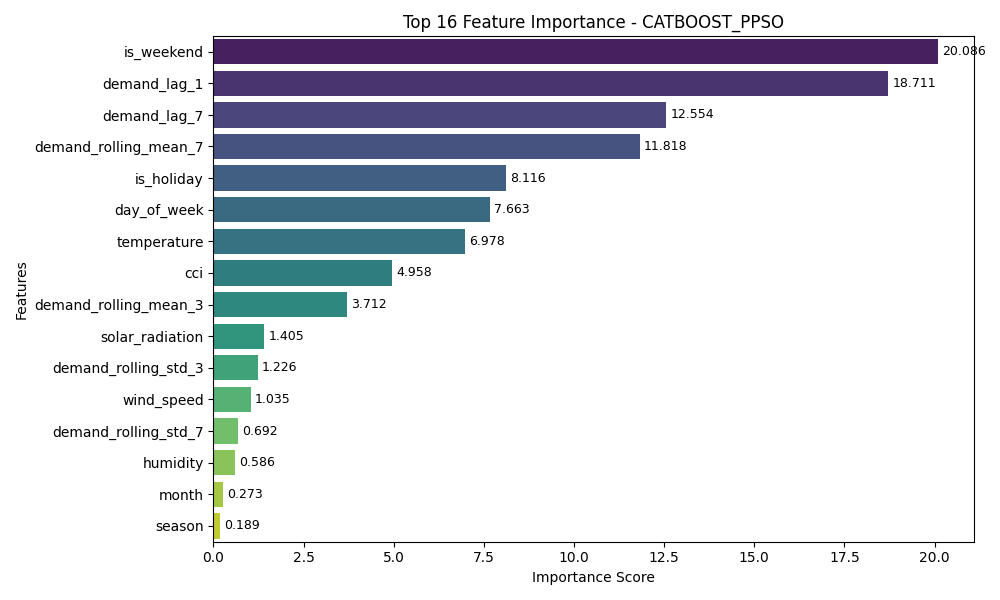
\includegraphics[width=0.85\textwidth]{eval/images/feature_importance_catboost_ppso.png}
    \caption{Feature importance scores from the CatBoost-PPSO model. The top features are autoregressive demand features, followed by weather and temporal variables.}
    \label{fig:feature_importance}
\end{figure}

\subsection{Interpretation of Feature Importance}

The feature importance ranking reveals a clear hierarchy:

\begin{enumerate}
    \item \textbf{Autoregressive features dominate}: \texttt{demand\_lag\_1} (yesterday's demand) is by far the most important predictor, consistent with the strong day-to-day autocorrelation of electricity demand. Rolling means (\texttt{demand\_rolling\_mean\_3}, \texttt{demand\_rolling\_mean\_7}) and \texttt{demand\_lag\_7} also rank highly, confirming that recent demand history is the strongest predictor of future demand.
    
    \item \textbf{Temporal features are significant}: \texttt{day\_of\_week} ranks prominently, reflecting the well-documented weekday/weekend demand differential. \texttt{month} and \texttt{season} capture longer-term temporal patterns.
    
    \item \textbf{Weather features contribute meaningfully}: \texttt{temperature} and \texttt{humidity} appear in the middle ranks, confirming their role as exogenous demand drivers. The \texttt{cci} (Comfort Climate Index) provides additional predictive value by capturing the combined thermal stress effect.
    
    \item \textbf{Wind speed and solar radiation} have lower but non-negligible importance, consistent with their indirect influence on cooling demand.
\end{enumerate}

\subsection{Comparison Across Models}

\begin{figure}[H]
    \centering
    \begin{subfigure}[b]{0.48\textwidth}
        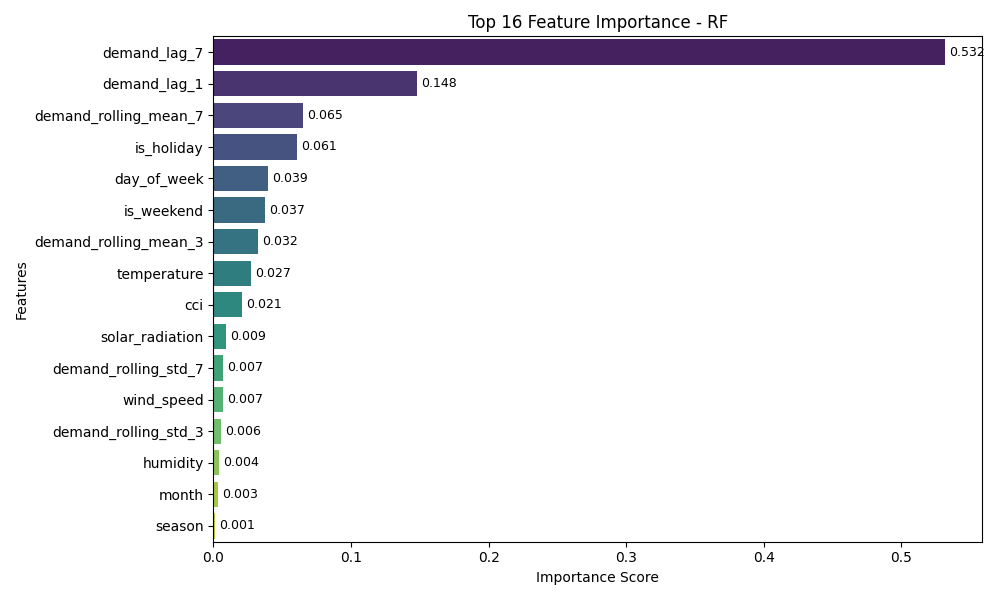
\includegraphics[width=\textwidth]{eval/images/feature_importance_rf.png}
        \caption{Random Forest}
    \end{subfigure}
    \hfill
    \begin{subfigure}[b]{0.48\textwidth}
        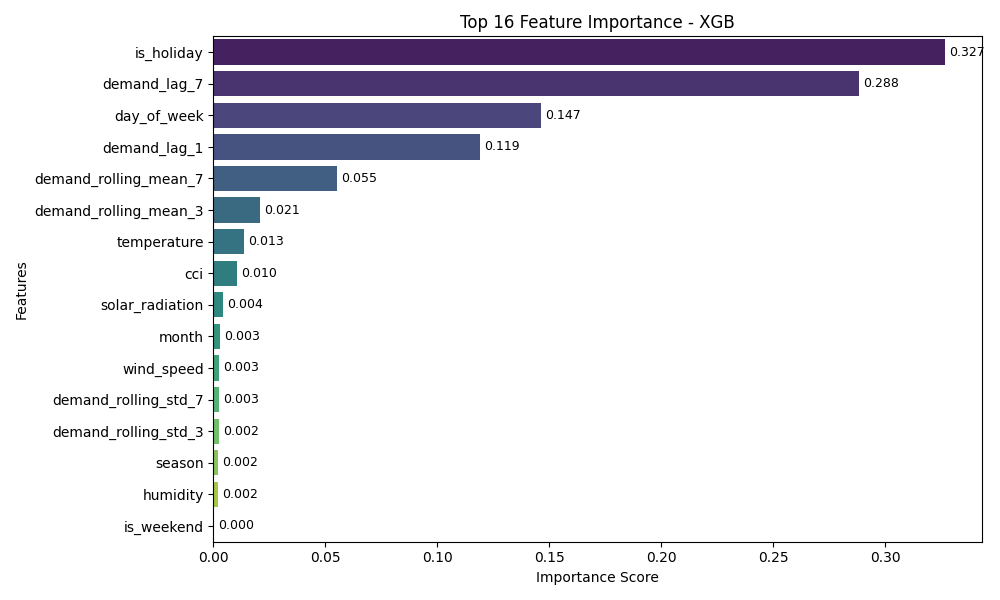
\includegraphics[width=\textwidth]{eval/images/feature_importance_xgb.png}
        \caption{XGBoost}
    \end{subfigure}
    \caption{Feature importance comparison between Random Forest and XGBoost. Both models agree on the dominance of autoregressive features.}
    \label{fig:feature_importance_comparison}
\end{figure}

The consistency of feature importance rankings across all tree-based models provides confidence that the identified feature hierarchy is robust and not an artefact of any single algorithm.


\section{Impact of PPSO Optimisation}

To quantify the impact of PPSO hyperparameter tuning, Table~\ref{tab:ppso_impact} compares each default tree model with its PPSO-optimised variant (RMSE and $R^2$), with CatBoost detailed across all metrics.

\begin{table}[H]
\centering
\caption{Impact of PPSO hyperparameter optimisation on CatBoost performance.}
\label{tab:ppso_impact}
\begin{tabular}{@{}lrrr@{}}
\toprule
\textbf{Metric} & \textbf{CatBoost (default)} & \textbf{CatBoost-PPSO} & \textbf{Improvement} \\
\midrule
MAE (MWh) & 1{,}679.4 & 1{,}496.2 & $-$10.9\% \\
RMSE (MWh) & 2{,}118.8 & 1{,}895.5 & $-$10.5\% \\
$R^2$ & 0.8919 & 0.9135 & $+$2.2 pp \\
MAPE (\%) & 0.99 & 0.89 & $-$10.6\% \\
RAE & 0.314 & 0.280 & $-$10.9\% \\
WI & 0.971 & 0.977 & $+$0.6 pp \\
\bottomrule
\end{tabular}
\end{table}

The PPSO-optimised CatBoost achieves approximately 10\% reduction in all error metrics and a 2.2 percentage-point improvement in $R^2$. XGBoost also gains from PPSO tuning (RMSE $-$6.4\%), while Random Forest does not (RMSE $+$2.1\%), showing that meta-heuristic tuning is not universally beneficial and its value depends on the sensitivity of the model family to its hyperparameters. This confirms the finding of Zhang et al.\ \parencite{zhang2023catboostppso} that PPSO is an effective meta-heuristic for CatBoost hyperparameter optimisation, and demonstrates that the approach generalises from hourly single-customer data to daily national-level demand in a different climate context.


\section{Comparison with Reference Study}

It is informative to compare the results of this project with those of the reference study by Zhang et al.\ \parencite{zhang2023catboostppso}. Table~\ref{tab:comparison_ref} presents a high-level comparison.

\begin{table}[H]
\centering
\caption{Comparison between this project and the reference study.}
\label{tab:comparison_ref}
\small
\begin{tabular}{@{}lll@{}}
\toprule
\textbf{Aspect} & \textbf{Zhang et al.\ (2023)} & \textbf{This Project} \\
\midrule
Temporal resolution & Hourly & Daily \\
Geographic context & Single residential customer & National (Singapore) \\
Climate & Not specified & Tropical equatorial \\
Data period & Dec 2010 -- Nov 2018 & Feb 2023 -- Dec 2025 \\
Best model RMSE & 42.3 (kW) & 1{,}895.5 (MWh) \\
Best model $R^2$ & 0.971 & 0.914 \\
Best model WI & 0.993 & 0.977 \\
No.\ of comparison models & 6 hybrid models & 8 configurations (incl.\ 3 PPSO-tuned) \\
\bottomrule
\end{tabular}
\end{table}

The lower $R^2$ in this project (0.914 vs.\ 0.971) is expected because daily national-level demand aggregates heterogeneous consumption patterns across millions of consumers, introducing more unexplained variance than a single household's consumption. Nevertheless, the results confirm that the CatBoost-PPSO methodology is effective across different scales and contexts.


\section{Discussion}\label{sec:discussion}

\subsection{Strengths of the Approach}

\begin{itemize}
    \item The automated PPSO tuning eliminates the need for manual hyperparameter selection, reducing human bias and the risk of sub-optimal configurations.
    \item The use of time-series cross-validation within the PPSO fitness function preserves temporal integrity and prevents overfitting to the training data.
    \item The 16-feature set captures multiple dimensions of demand variation (weather, calendar, historical), resulting in consistently high $R^2 > 0.87$ across all models.
    \item CatBoost's native categorical handling is advantageous for the multi-type feature set used in this project.
\end{itemize}

\subsection{Limitations and Potential Sources of Error}

\begin{itemize}
    \item \textbf{Data resolution}: Daily aggregation masks intra-day demand peaks, which are critical for operational grid management.
    \item \textbf{Weather data quality}: Open-Meteo provides reanalysis data that may differ from actual ground-station measurements.
    \item \textbf{External events}: The model does not account for economic shocks, major infrastructure changes, or COVID-19 residual effects on demand patterns.
    \item \textbf{PPSO stochasticity}: Despite fixing the random seed, the stochastic nature of PPSO means that different runs may converge to slightly different hyperparameter configurations.
\end{itemize}


\section{Conclusions}

The evaluation demonstrates that the CatBoost-PPSO model achieves the best predictive performance among all tested model configurations, with an $R^2$ of 0.914, MAE of 1{,}496.2 MWh, and MAPE of 0.89\%. PPSO optimisation provides a consistent $\sim$10\% improvement over default CatBoost across all error metrics, a smaller gain for XGBoost, and no gain for Random Forest---evidence that the fair, uniform tuning protocol correctly isolates algorithmic merit. Feature importance analysis confirms that autoregressive demand features are the strongest predictors, with temperature and temporal calendar features providing important supplementary signal. These results validate the applicability of the hybrid CatBoost-PPSO methodology to daily national-level demand forecasting in a tropical climate.
